\section{閉曲線の正 normal shell と一価頂点のない分岐 graph}
\label{ncb:section}

本節では、閉じた平面切断曲線の全体を使う別の actual block を構成する。
その曲線方向の基底には一価の頂点がなく、特異 fibers は corank-one hyperbolic 型のみである。
Normal moment の有限 window による側面は残る。
前節までの24個の annular collars を固定する相対定理でも、48本の新 regular ports を
接続したという主張でもない。閉曲線の topology と非自明な normal bundle を同時に使う
構成を、今後の接続に使える独立の出発点として与える。

\subsection{極大・極小を持たない circle-valued Morse map}

次の曲面論の事実自体は既知である。
例えば de Rezende--Ledesma--Manzoli Neto--Vago の
\cite[Theorem 5.5, Lemma 5.7]{circle-morse-ncb}を参照されたい。
本稿では必要な genus と whole fibers を明示するため、pants の接着から構成する。

\begin{lemma}[一価頂点のない Reeb graph]\label{ncb:circle-morse}
$C$ を genus $g\ge2$ の closed connected oriented smooth surface とする。
Critical values が互いに異なる smooth map $f:C\to\RR/\ZZ$ を、
critical points がちょうど $2g-2$ 個で全て index one となるよう選べる。
その connected-level quotient $q:C\to\Gamma$ は finite connected Hausdorff graph であり、
\begin{equation}\label{ncb:graph-counts}
 \#V(\Gamma)=2g-2,\qquad
 \#E(\Gamma)=3g-3,\qquad b_1(\Gamma)=g.
\end{equation}
全 vertices は三価で、regular fibers は circles、vertex fibers は figure-eights である。
\end{lemma}

\begin{proof}
一つの incoming circle と二つの outgoing circles を持つ elementary pair of pants に、
唯一の critical point が index one である height function を入れる。
局所式 $x^2-y^2$ に regular collars を付加すればよい。
二つの incoming circles を一つに merge する逆向きの pants と、二本の中間 cuffs で接ぐ。
Boundary collars の height coordinates を一致させ、induced boundary orientations に関して
逆向きに接着することで、genus one、boundary 二つの oriented cobordism $B$ を得る。
Height は両端 collar で product coordinate となり、内部には split と merge の二つの saddles だけがある。

$n=g-1$ 個の $B_j$ を取り、height の値域を順に
$[j/n,(j+1)/n]$ とする（添字 $j=0,\ldots,n-1$）。
Outgoing circle と次の incoming circle を、height の product collars を保って接ぎ、
最後も最初へ巡回的に接ぐ。
値域の両端を modulo $1$ で同一視すると、滑らかな circle-valued map を得る。
各 $B_j$ の二つの critical values は、その区間の内部で全て異なるように選ぶ。
Seam の近くは product なので新しい critical points は生じない。
得られた surface は closed、connected、oriented であり、
\[
 \chi=\sum_{j=0}^{n-1}\chi(B_j)=-2n=2-2g.
\]
従って genus $g$ の $C$ へ orientation-preserving diffeomorphism で移せる。

各 $B_j$ の quotient は、二つの trivalent vertices を二本の parallel edges で結び、
それぞれに incoming と outgoing の cuff edge を持つ graph である。
巡回接着後、vertices は $2n$ 個、二本ずつの中間 edges が $2n$ 本、
隣接 $B_j$ を結ぶ edges が $n$ 本なので、$E=3n$ である。
Connected graph の $b_1=E-V+1$ より $b_1=n+1=g$ を得る。
この有限 graph への quotient は、pants と regular cylinders の connected-level quotients を
有限個接いだものなので Hausdorff である。Singular level は各 pants の figure-eight である。
\end{proof}

\begin{lemma}[可縮な regular level はない]\label{ncb:essential-circles}
Closed surface 上の circle-valued Morse map が extrema を持たなければ、
その regular level の各 circle component は surface 内で非可縮である。
\end{lemma}

\begin{proof}
可縮な embedded circle は disk $D$ を bound する。
$f|_D$ は $D$ の単連結性から実数値関数 $F$ へ lift でき、$F|_{\partial D}$ は定数である。
$F$ が非定数なら、境界値との大小に応じて interior maximum または minimum を持つ。
これは $f$ の extrema となる。$F$ が定数なら open disk 上に critical points があり、Morse 条件に反する。
\end{proof}

特に、閉曲線 $C^*$ の24個の削除円板の小さい境界 circles を、
この $f$ の regular level components として同時に保持することはできない。
この補題は base curve の circles に関する主張であり、
ambient 六次元多様体内の新しい regular ports の一般的接続を排除するものではない。

\subsection{平面切断曲線の global normal model}

以後 $X_d\subset\PP^4$ を smooth hypersurface、$d\ge6$、
$\omega$ を所定の K\"ahler form、$[\omega]=\mathfrak a\mathsf H$, $\mathfrak a>0$ とする。
二つの generic hyperplanes による切断を $C$ とすれば、$C$ は smooth plane curve of degree $d$ であり、
\begin{equation}\label{ncb:curve-data}
 g(C)=\frac{(d-1)(d-2)}2,\qquad
 \int_C\omega_C=d\mathfrak a,\qquad
 N_{C/X_d}\simeq\mathcal O_C(1)\oplus\mathcal O_C(1),
 \quad\omega_C=\omega|_C.
\end{equation}
Smoothness は generic hyperplane sections、normal bundle は二つの transverse equations の
conormal sequence から従う。Genus は $K_C\simeq\mathcal O_C(d-3)$ から得られる。
六次の既存 pencil では、命題\ref{ad:fixed-curve}の固定曲線 $C^*$ をそのまま使える。

Symplectic normal bundle を compatible complex structure と metric で complex rank two bundle と見て、
上の二つの line summands に対応する symplectically orthogonal splitting $L_1\oplus L_2$ を選ぶ。
第一の complex line とその Hermitian complement を取る方法でも、
第二の quotient line が $\mathcal O_C(1)$ と同型なので実現できる。
元の二つの非直交な complex normal lines を同時に固定することは要求しない。

角の周期は $1$、fiberwise actions は $p_j=\pi|z_j|^2$ とする。
Unit circle bundle $P(L_j)$ の connection $\alpha_j$ は
$\alpha_j(\partial_{\theta_j})=1$ と規格化し、
\begin{equation}\label{ncb:connections}
 d\alpha_j=\pi^*\kappa_j,
 \qquad [\kappa_j]=-c_1(L_j),
 \qquad \kappa_1=\kappa_2=-\frac{\omega_C}{\mathfrak a}
\end{equation}
となるよう選ぶ。最後の curvature form の積分は $-d$ で、所要の class と一致する。
任意の connection の curvature との差は exact なので、base one-form を加えてこの選択ができる。

Normal bundle の zero section の近傍に
\begin{equation}\label{ncb:omega}
 \begin{split}
 \Omega_N
 &=\pi^*\omega_C+\sum_{j=1}^2 d(p_j\alpha_j)\\
 &=\left(1-\frac{p_1+p_2}{\mathfrak a}\right)\pi^*\omega_C
       +dp_1\wedge\alpha_1+dp_2\wedge\alpha_2
 \end{split}
\end{equation}
を入れる。$p_j\alpha_j$ は $z_j=0$ へも滑らかに延びる。
Connection による horizontal--vertical splitting から、$p_1+p_2<\mathfrak a$ で symplectic であり、
zero section 上では所定の tangent form と normal fiber form に一致する。

\begin{lemma}[閉曲線全体に沿う actual normal embedding]\label{ncb:embedding}
ある $\varepsilon>0$ に対し、$p_1+p_2<\varepsilon$ の normal disk bundle から
$(X_d,\omega)$ への symplectic embedding $\Psi$ があり、zero section 上で $C$ への恒等写像となる。
その normal first jet は、選んだ symplectic normal bundle の同定と一致させられる。
$\varepsilon<\mathfrak a$ としてよい。
\end{lemma}

\begin{proof}
Zero section とその normal first jet を指定して smooth tubular embedding $F$ を取る。
$F^*\omega$ と $\Omega_N$ は zero section 上で full bilinear forms として一致する。
Normal radial homotopy による difference の primitive は $O(|z|^2)$ であり、
十分小さい disk bundle 上では両形式の直線補間が symplectic である。
Relative Moser field は zero section と normal first jet を固定する。
Compact な $C$ 全体に対して共通の radius を選び、その time-one map と $F$ を合成する。
これは symplectic neighborhood theorem の直接の relative Moser 証明である
\cite[Section 7.3, Theorem 7.4]{cds-local}。
所定の K\"ahler form 自体を変更するのではなく、模型からその form への symplectic embedding を作っている。
\end{proof}

\subsection{全曲線上の actual hyperbolic torus block}

\begin{theorem}[一般次数に対する一価頂点のない曲線方向の block]\label{ncb:actual-block}
式\eqref{ncb:curve-data}の $C\subset X_d$ に対し、十分小さい compact rectangle
\[
 P=[p_1^-,p_1^+]\times[p_2^-,p_2^+],
 \qquad 0<p_j^-<p_j^+,\qquad p_1^++p_2^+<\varepsilon
\]
を取る。Normal bundle 内の shell
\[
 \mathcal A_P=\{(z_1,z_2)\in L_1\oplus L_2:(p_1,p_2)\in P\}
\]
の actual image $\Psi(\mathcal A_P)\subset X_d$ 上に、connected Lagrangian fibers を持つ map
\begin{equation}\label{ncb:fibration}
 \Pi:\Psi(\mathcal A_P)\longrightarrow P\times\Gamma
\end{equation}
がある。$\Gamma$ は補題\ref{ncb:circle-morse}の一価頂点のない graph であり、
\begin{equation}\label{ncb:d-counts}
 \#V=d(d-3),\qquad
 \#E=\frac{3d(d-3)}2,\qquad
 b_1(\Gamma)=\frac{(d-1)(d-2)}2.
\end{equation}
Regular fibers は $T^3$、vertex fibers は $T^2\times(S^1\vee S^1)$ である。
各 vertex 上には $P$ で parameterize された nondegenerate rank-two hyperbolic orbit の族があり、
elliptic fibers は存在しない。Base は Hausdorff であり、曲線方向に free boundary はない。
一方 $\partial P\times\Gamma$ に沿う normal-action faces は残る。
\end{theorem}

\begin{proof}
模型上で
\[
 \Pi_N(z_1,z_2)=\bigl(p_1,p_2,q(\pi(z_1,z_2))\bigr)
\]
と定め、$\Psi$ で運ぶ。
Normal rotations は $\iota_{\partial_{\theta_j}}\Omega_N=-dp_j$ を満たす free Hamiltonian $T^2$ action である。
Circle-valued $f$ の各 local real lift $F$ に対し、$F\circ\pi$ は rotations に invariant なので、
$p_1,p_2,F\circ\pi$ は互いに Poisson commute する。
Regular point ではこれらの differentials は独立である。

Fixed $p=(p_1,p_2)$ の reduction は $C$ であり、その symplectic form は
\begin{equation}\label{ncb:reduction}
 \omega_p=\left(1-\frac{p_1+p_2}{\mathfrak a}\right)\omega_C.
\end{equation}
Regular circle $\gamma=q^{-1}(b)$ の inverse image 上では $dp_j=0$ である。
Base へ射影した tangent space は一次元なので、$\omega_C$ も curvature terms もそこで零になる。
従って inverse image は三次元 Lagrangian である。
Principal $T^2$ bundle の circle 上の制限は $H^2(S^1;\ZZ^2)=0$ により trivial であり、fiber は $T^3$ となる。

Critical point では $F$ の reduced Hessian が index one であり、$p_j$ の二つの free orbit directions と合わせて
nondegenerate corank-one hyperbolic 型になる。
Vertex の whole level component は figure-eight である。
その上でも $H^2(S^1\vee S^1;\ZZ^2)=0$ なので、principal bundle の制限は trivial であり、
whole singular fiber は $T^2\times(S^1\vee S^1)$ である。
この議論に $L_j$ の $C$ 全体での triviality は不要である。

各 fiber は connected で、compact source から compact Hausdorff space $P\times\Gamma$ への continuous surjection なので
表示は connected-fiber quotient である。
Formula \eqref{ncb:d-counts} は式\eqref{ncb:graph-counts}と genus formula の代入から従う。
Normal moments が正のため axes は domain に含まれず、$f$ に extrema がないため elliptic fibers はない。
\end{proof}

六次では、$g=10$、$\#V=18$、$\#E=27$、$b_1=10$ である。
この18は新しい shell の hyperbolic families の数であり、従来の24 caps からの families とは別の構成である。
両者を自動的に加算して一つの actual assembly の特異 fibers の数としてはならない。

\begin{figure}[htbp]
\centering
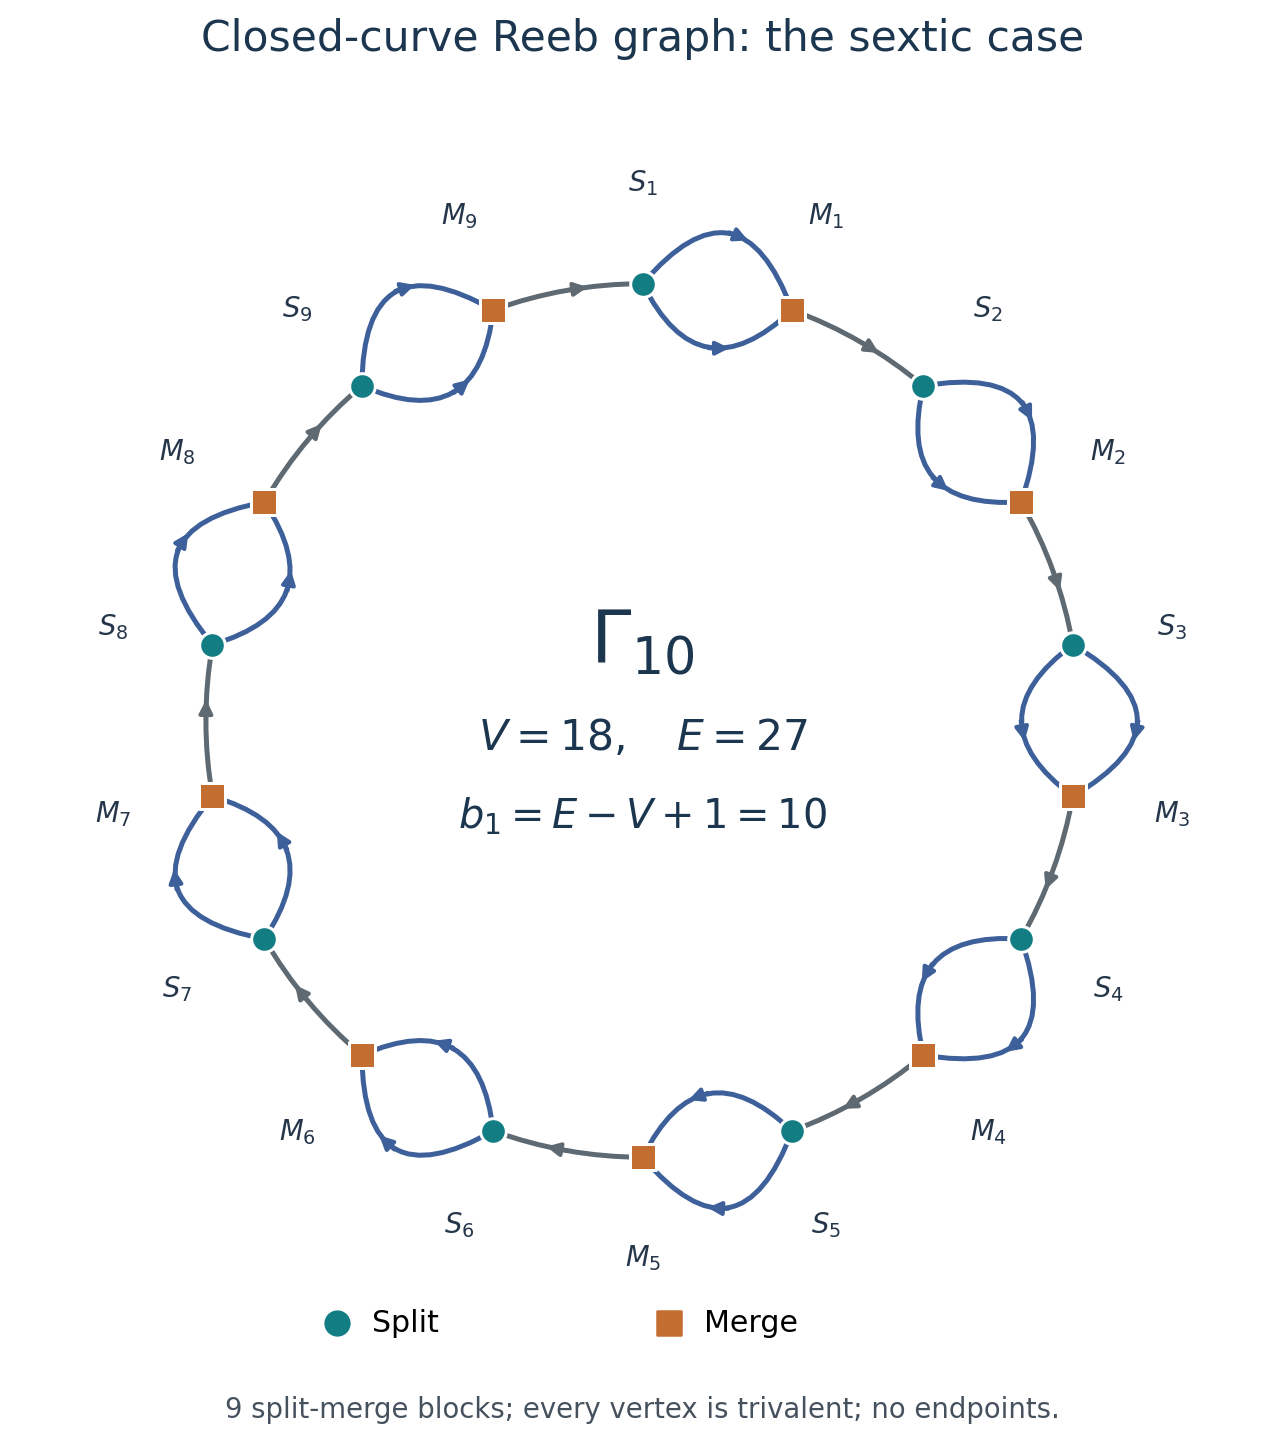
\includegraphics[width=0.83\textwidth]{closed_curve_graph.png}
\caption{六次の閉曲線に対する circle-valued Morse map の Reeb graph。
9個の split--merge cobordisms を巡回接着し、18頂点、27辺、$b_1=10$ を得る。
全頂点は三価である。Actual block の三次元基底は、この graph と二つの normal actions の
rectangle $P$ との積であり、$\partial P$ の側面は図示していない。}
\label{ncb:graph-figure}
\end{figure}

\paragraph{接続への意味と限界.}
この構成では、閉曲線の一周方向を circle-valued map にすることで、
曲線方向の extrema を最初から作らない。
ただし domain は zero section と二つの normal axes を含まず、normal moments の上下 faces も未接続である。
旧 curve block の transverse focus foliation と、ここで使う二つの normal rotations は異なる選択である。
24個の既定 annular germs、primitive constants、new pants ports との一致はこの定理の結論に含めない。
特に補題\ref{ncb:essential-circles}により、旧 puncture の contractible base cuffs をこの $f$ の
regular levels のまま保持することはできない。
既存48 ports との接続には、実際の overlap、period lattice と boundary coorientation の比較が必要である。
また二つの normal circles はこの shell には存在するが、系\ref{gc:hypersurface}により
全 $X_d$ の非自明な symplectic circle action として延長することはできない。

\subsection{Section を持たない閉還元面の Euler 補正}

前節の構成では、closed reduced surface は $C$ であるが、principal $T^2$ bundle の
Chern vector は $(d,d)$ であり section は存在しない。
従って系\ref{rsb:closed-section}を無条件には適用できない。
ここで必要な一般式を示す。

$(X,\omega)$ を simply connected symplectic six-manifold とし、
\[
 [\omega]+\nu c_1(TX)=0,\qquad\nu>0
\]
と仮定する。Shared orbit の boundary covector は、式\eqref{rsb:theta}で $\mathfrak a$ を $\nu$ に置換し、
\[
 \Theta_L(v)=\operatorname{Area}(D)+\frac\nu2\mu(D)
\]
と定める。前節と同じ comparison により well-defined であり、同じ free Hamiltonian $T^2$ の
同じ moment level 上で shared restriction $\Theta_\Gamma$ は一定である。

\begin{proposition}[閉還元面の面積・Euler class 収支]\label{ncb:closed-budget}
一つの regular moment level 内の compact free $T^2$-invariant submanifold $E$ の reduction を
closed connected oriented surface $\Sigma$ とする。
固定 generators に関する principal bundle の Chern vector を
\[
 c=(c_1,c_2)\in\ZZ^2,\qquad
 c_j=-\int_\Sigma\kappa_j
\]
とする。ここで $\alpha_j(\Gamma_k)=\delta_{jk}$、$d\alpha_j=\pi^*\kappa_j$ であり、
unit circle bundle of a complex line では $c_j$ はその line の degree である。
このとき
\begin{equation}\label{ncb:closed-budget-equation}
 \boxed{\quad
 \operatorname{Area}(\Sigma)+\nu\chi(\Sigma)+\Theta_\Gamma(c)=0.
 \quad}
\end{equation}
\end{proposition}

\begin{proof}
Small closed disk $D\subset\Sigma$ を取り、$\Sigma_0=\Sigma\setminus\operatorname{int}D$ とする。
両者の上に sections $s_D,s_0$ がある。
$v=\partial s_D(D)$ は正向きの base disk boundary を射影し、
area $A_D=\operatorname{Area}(D)>0$、Maslov index $2$ を持つ。
後者は補題\ref{rsb:maslov-section}の free orbit framing の証明を disk に適用して得られる。
Boundary torus 上で
\[
 [s_0(\partial\Sigma_0)]=-[v]+m_1\Gamma_1+m_2\Gamma_2
\]
と書く。$\alpha_j$ はこの boundary torus 上では closed であり、Stokes より
\[
 m_j
 =\int_{s_0(\partial\Sigma_0)}\alpha_j+\int_v\alpha_j
 =\int_{\Sigma_0}\kappa_j+\int_D\kappa_j
 =-c_j.
\]
従って式\eqref{rsb:full-budget}の $\nu$ 版を $\Sigma_0$ に適用すると
\[
 \operatorname{Area}(\Sigma_0)+\nu\chi(\Sigma_0)
 =-(A_D+\nu)-\Theta_\Gamma(c).
\]
$\chi(\Sigma_0)=\chi(\Sigma)-1$ と面積の加法性から結論を得る。
\end{proof}

\begin{corollary}[Normal shell の全次数の収支]\label{ncb:normal-budget}
定理\ref{ncb:actual-block}において $\nu=\mathfrak a/(d-5)$ と置く。
Positive normal rotations の reference disks は面積 $p_j$、Maslov index $2$ を持つので
\begin{equation}\label{ncb:normal-theta}
 \Theta_\Gamma(e_1,e_2)=e_1(p_1+\nu)+e_2(p_2+\nu).
\end{equation}
Reduction の area、Euler characteristic、Chern vector は
\begin{equation}\label{ncb:normal-numbers}
 \operatorname{Area}(C_p)=d(\mathfrak a-p_1-p_2),\qquad
 \chi(C)=d(3-d),\qquad c=(d,d).
\end{equation}
これらは式\eqref{ncb:closed-budget-equation}を満たす。
\end{corollary}

\begin{proof}
Reference disk は base point と他方の normal coordinate を固定し、$z_j$ の半径を零まで縮める
fiber disk である。Area は $p_j$、boundary tangent の一回転から Maslov index は $2$ である。
他の tangent directions はこの disk 上で framing されている。
Area formula は式\eqref{ncb:reduction}の積分、Euler characteristic は genus formula、
Chern vector は $\deg L_j=d$ から得られる。
全てを代入すると
\[
 \begin{split}
 &d(\mathfrak a-p_1-p_2)+\nu d(3-d)
       +d(p_1+p_2+2\nu)\\
 &\hspace{20mm}=d\mathfrak a+\nu d(5-d)=0.
 \end{split}
\]
従って、nontrivial normal bundle の Euler correction を含めると負の単調性と厳密に整合する。
\end{proof}

六次では reduction の面積は $6(\mathfrak a-p_1-p_2)$ であり、
section を持つ genus $10$ reduction の式 $18\mathfrak a$ とは異なる。
その差を担うのが $\Theta_\Gamma(6,6)=6(p_1+p_2+2\mathfrak a)$ である。
この補正は arbitrary gluing の存在を与えるものではないが、
閉曲線近傍に実際に存在する reduction を誤って除外しないために必要である。


\subsection{Zero section の coherent focus 充填への制約}

% Short application of existing lc:framing:hessian / lc:framing:chern.
% No new obstruction principle is claimed.
\paragraph{Zero section を全て同じ focus subsystem で埋めることへの制約.}
定理\ref{ncb:actual-block}の positive normal shell は zero section と normal axes を含まない。
これらを追加するとき、既存の tensor-line 障害
（補題\ref{lc:framing:hessian}、命題\ref{lc:framing:chern}）は次の形になる。

\begin{corollary}[Closed normal curve に沿う coherent focus の障害]
\label{ncb:closed-focus-obstruction}
$L_1\oplus L_2=N_{C/X_d}$、$L_j\simeq\mathcal O_C(1)$ とし、
normal circle を $H=p_1-p_2$ に固定する。
Zero section $C$ に沿う smooth real transverse integral $Q$ があり、
$Q|_C=0$、$\{H,Q\}=0$、かつ $H$ と $Q$ の normal quadratic pair が
$C$ の全点で nondegenerate focus--focus 型となることはない。
同じ結論は、global $Q$ の代わりに local generators $Q_a$ を使い、その normal quadratic parts が
\[
 [Q_a]=a_{ab}[Q_b]\pmod{\mathbb R H},\qquad a_{ab}\in\mathbb R^\times
\]
と変換する coherent transverse subsystem にも成り立つ。
\end{corollary}

\begin{proof}
$H$ は normal fibers に weights $(+1,-1)$ で作用する。
$Q|_C=0$ と invariance により $dQ|_C=0$ であり、normal Hessian は内在的に定まる。
$r_j=|z_j|^2/2$ と書き、$H$ の倍と正の period normalization を除けば
\[
 Q_2=t(r_1+r_2)+\operatorname{Re}(b z_1z_2)
\]
となる。Invariant quadratic monomials は $|z_1|^2,|z_2|^2,z_1z_2,\bar z_1\bar z_2$ だけである。
補題\ref{lc:framing:hessian}により focus 条件は $|b|^2>t^2$、特に $b\ne0$ を必要とする。
しかし $b$ は
\[
 (L_1\otimes L_2)^*\quad\text{の切断であり}\quad
 \deg((L_1\otimes L_2)^*)=-2d\ne0
\]
なので nowhere-zero section にはなれない。
Local real-generator transitions の場合も命題\ref{lc:framing:chern}により
$2c_1(L_1\otimes L_2)=0$ が必要であり、$H^2(C;\mathbb Z)\simeq\mathbb Z$ では不可能である。
\end{proof}

Smooth coefficient $b$ が zero section に transverse なら、その零点の局所指数は $\pm1$ であり、
符号付き総和は $-2d$ である。従って零点数は少なくとも $2d$ であるが、
一般にはちょうど $2d$ とは限らない。
これは mixed quadratic coefficient の零点に関する数であり、
必要な global singular fibers の個数、あるいは non-focus locus 全体の点数ではない。
実際、diagonal term $t$ が非零なら $|b|^2\le t^2$ の領域も focus 条件を満たさない。

この系は、positive normal shell 自体や、local focus neighborhoods、
vanishing circle / weight splitting / transverse subsystem を変更する completion を排除しない。
新しい shell の zero section 全体を fixed coherent focus family で一括して埋める工程に対する必要条件である。
新規な一般原理としてではなく、既存 tensor-line 障害の closed actual curve への適用として位置付ける。
